\section*{Consigna}

Se quiere enviar un paquete de 1600 B de payload desde \textbf{A} hasta \textbf{B} utilizando IPv4 a través de una red cuya topología se muetra a continuación. DF inicial es 0.

\begin{figure}[H]
    \centering
    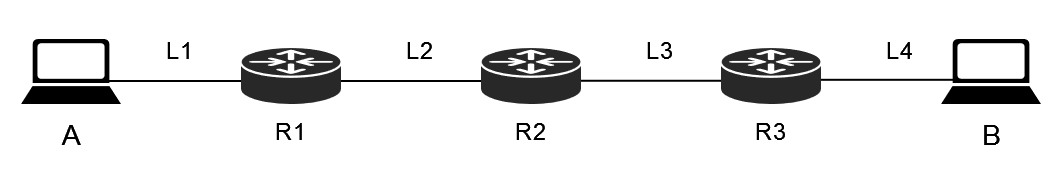
\includegraphics[width=0.9\linewidth]{Images/topologia.png}
\end{figure}

\vspace{-5mm}
{
\renewcommand{\arraystretch}{1.5}
\begin{table}[H]
    \centering
    \begin{tabular}{|c|c|c|c|c|}
    \hline
     & L1 & L2 & L3 & L4 \\ \hline
    MTU (B) & 2000 & 1000 & 800 & 2000\\ \hline
    \end{tabular}
\end{table}
}


\begin{enumerate}
    \item Llenar la siguiente tabla con todos los paquetes que lleguen al host:

    \begin{table}[H]
    \centering
    \renewcommand{\arraystretch}{1.5}
    \begin{tabular}{|c|c|crrrrr|}
    \hline
    \multirow{2}{*}{Name} & \multirow{2}{*}{Payload Size} & \multicolumn{6}{c|}{Datagram Header} \\ \cline{3-8} 
     &  & \multicolumn{1}{c|}{IHL} & \multicolumn{1}{c|}{Total Length} & \multicolumn{1}{c|}{ID} & \multicolumn{1}{c|}{MF} & \multicolumn{1}{c|}{DF} & \multicolumn{1}{c|}{Fragment Offset} \\ \hline
    \multicolumn{1}{|r|}{} & \multicolumn{1}{r|}{} & \multicolumn{1}{r|}{} & \multicolumn{1}{r|}{} & \multicolumn{1}{r|}{} & \multicolumn{1}{r|}{} & \multicolumn{1}{r|}{} &  \\ \hline
    \multicolumn{1}{|r|}{} & \multicolumn{1}{r|}{} & \multicolumn{1}{r|}{} & \multicolumn{1}{r|}{} & \multicolumn{1}{r|}{} & \multicolumn{1}{r|}{} & \multicolumn{1}{r|}{} &  \\ \hline
    \end{tabular}
    \end{table}

    \item ¿Llegarían los mismos fragmentos si se quisiera enviar el mismo paquete desde \textbf{B} hacia \textbf{A}?
    
    \item ¿Qué pasaría si el DF inicial fuera 1?
    
    \item ¿Podría reensamblarse el paquete en el último router?
    
    \item ¿Qué pasa si se pierde uno de los fragmentos?
    
    \item ¿Qué pasa si llegan desordenados?
\end{enumerate}
